\section{Prototyp programu}
\subsection{Wykorzystane moduły}
Przed przystąpieniem do pracy nad algorytmem, użyliśmy biblioteki \textbf{WFDB} dla środowiska MATLAB, która umożliwiła pobranie danych EKG z bazy MIT-BIH\cite{mit-bih}.

W prototypowej wersji programu użyliśmy modułu \textbf{NumPy} do operacji na macierzach i operacji numerycznych, w tym: interpolacji wielomianowej, sklejania i obracania wektorów. 
Moduł matplotlib.pyplot posłużył do obrazowania wyników.

\subsection{Oprogramowanie algorytmu}
Ponieważ odpowiedź impulsowa filtru $h$ jest niezależna od wartości sygnału, wartości wektora $h$ o długości $2M+1$ wystarczy obliczyć raz, a następnie obliczyć wartość konwolucji sygnału z taką maską. Wartości maski zostały pokazane na rysunku \ref{rys:impuls}.

\begin{figure}[!htb]
  \begin{center}
    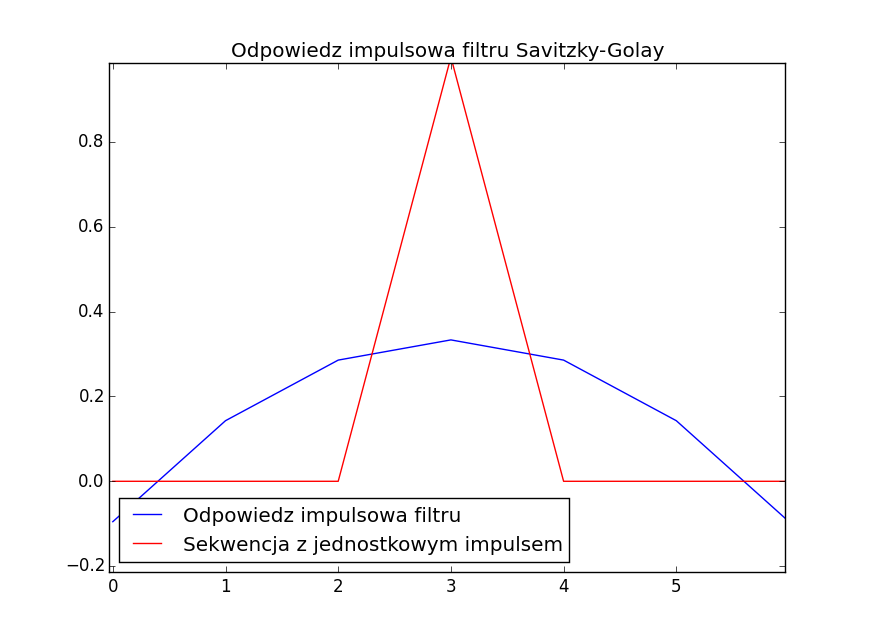
\includegraphics[scale=0.8]
    {img/impulse.png}
  \end{center}
  \caption{Odpowiedź impulsowa filtru, uzyskana jako interpolacja wielomianem $N=2$ stopnia serii $2M+1=7$ próbek z jednostkowym impulsem pośrodku}
  \label{rys:impuls}
\end{figure}

\subsection{Wartości brzegowe}
Algorytm w każdym punkcie potrzebuje do obliczeń $M$ punktów z lewej i $M$ punktów z prawej strony, zatem należy zdecydować o zachowaniu programu na początku i na końcu spróbkowanego sygnału.

Istnieje kilka możliwych rozwiązań:
\begin{enumerate}
\item Zawijanie - algorytm wykorzysta pierwsze $M$ punktów na końcu oraz ostatnie $M$ punktów na początku sygnału
\item Odbicie - na brzegach zostaną wykorzystane najbliższe punkty, jednak w odwróconej kolejności
\item Użycie stałej, ustalonej wartości
\item Najbliższy sąsiad - poza granicami sygnału zostaną dopisane punkty równe pierwszej próbce (na początku) i ostatniej próbce (na końcu)
\end{enumerate}

W prototypie wybraliśmy rozwiązanie 2. Jeśli ostatnie punkty mają wartości $[6, 7, 8, 9]$, to dopisane poza prawą granicą punkty otrzymają wartości $[8, 7, 6]$.


Przebieg filtracji zakłóceń o wysokiej częstotliwości uzyskanej za pomocą prototypu Python przedstawia wykres \ref{rys:savitzky_py}.

\begin{figure}[!htb]
  \begin{center}
    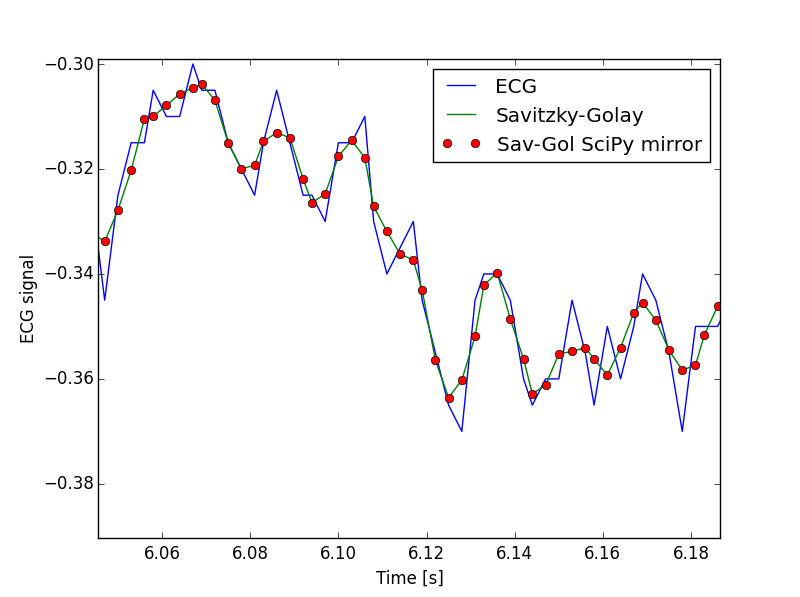
\includegraphics[scale=0.8]
    {img/prototype.png}
  \end{center}
  \caption{Wygładzanie metodą Savitzky-Golay z oknem 7 próbek (M=3) i aproksymacją wielomianem N=2 stopnia. Porównanie prototypu z funkcją z modułu SciPy.signals}
  \label{rys:savitzky_py}
\end{figure}

\subsection{Usunięcie szumu o niskiej częstotliwości}

Przyjmując dużą szerokość okna filtracji, z sygnału EKG odrzucono wysokie częstotliwości, łącznie z kompleksami QRS i pozostałymi charakterystycznymi zmianami wartości sygnału. Otrzymano w ten sposób izolinię, którą następnie usunięto, odejmując jej wartości od sygnału EKG. Rysunek \ref{rys:remove} przedstawia wyniki usunięcia izolinii dla okna $M=500$ przy aproksymacji wielomianem $N=2$ stopnia.

\begin{figure}[!htb]
  \begin{center}
    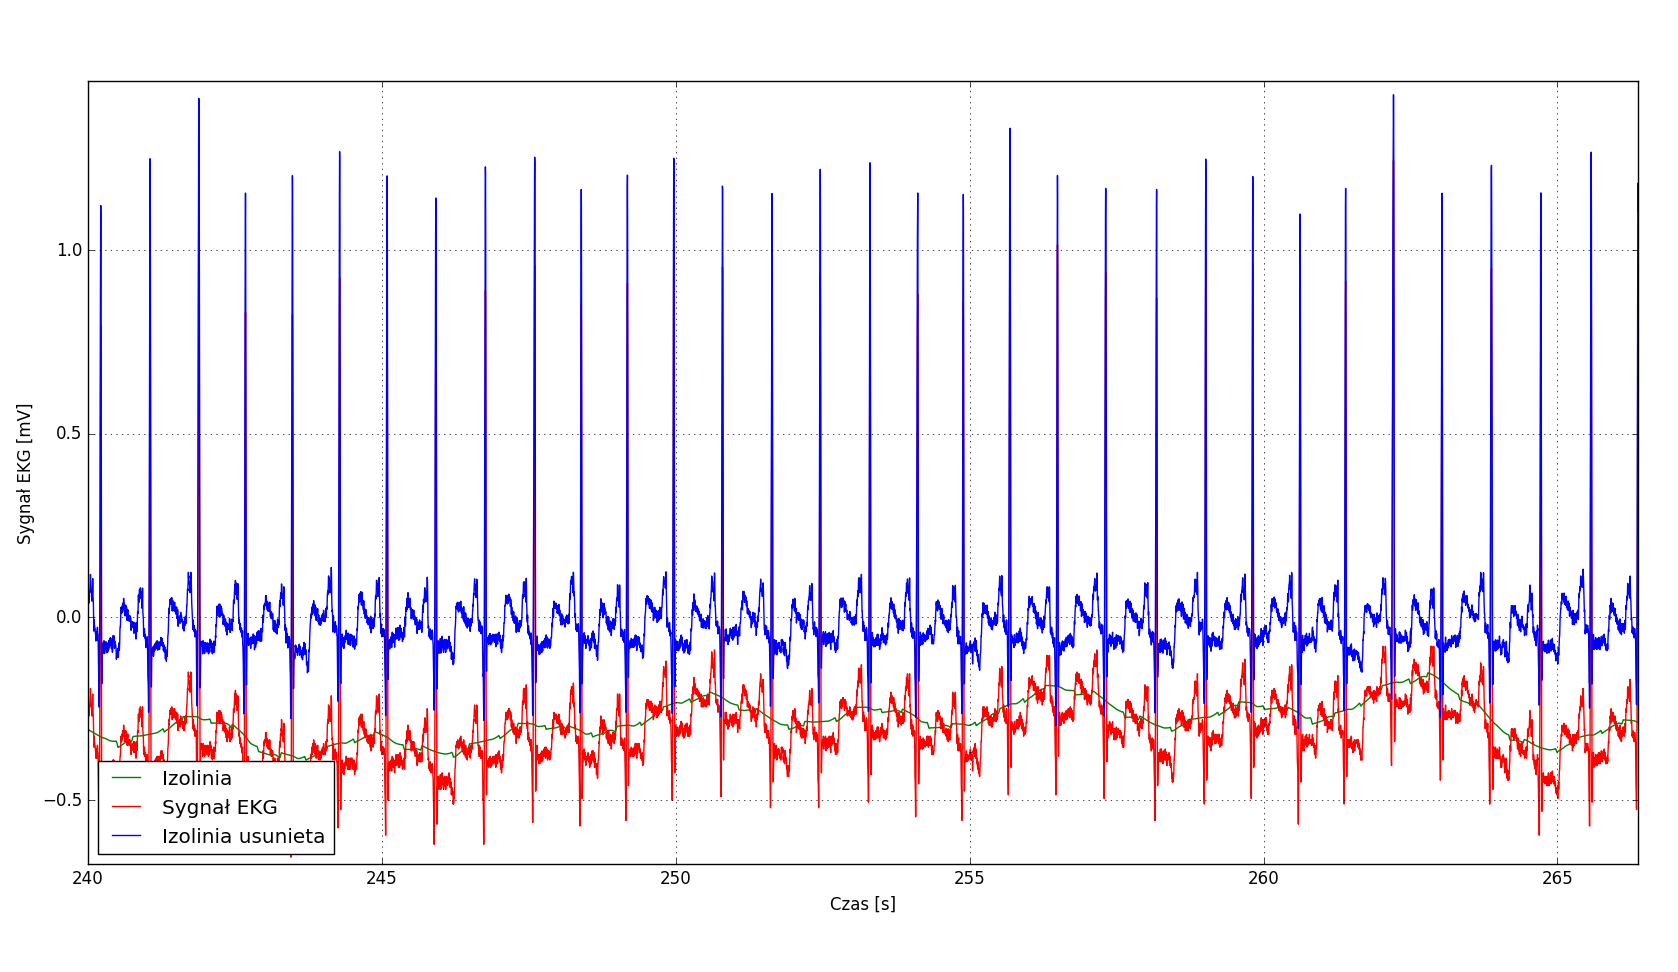
\includegraphics[scale=0.4]
    {img/remove_baseline1.png}
  \end{center}
  \caption{Wykrycie i usunięcie izolinii sygnału EKG z użyciem filtra Savitzky-Golay o parametrach $M=500$, $N=2$}
  \label{rys:remove}
\end{figure}
